\chapter{Discussion}

In this chapter the technical results of the project are analyzed. First, the design verification is performed, comparing the simulation and the experimental results. Then, the main drawbacks found through the project and limitations of the converter are explained. Finally, suggestions for future work are presented.

\section{Verification of experimental results} \label{Experiment_verification}
In this section the experimental results from the open-loop and MPPT test in section \ref{systemtest} are compared with the simulation results from section \ref{sec:componentsizing} and \ref{MPPTSimulation}.

\subsection{Open-loop simulation} \label{ol_discussion}

%The main losses are the dissipation from the component in heat. Also the load is a power resistor and it changes the resistance if it is in operation. So we have not a constant load at the output as in the simulation. Another reason is the dead-time of the MOSFET and therefore the duty cycle is not exactly the same value as in the simulation. belongs to the topic between efficiency simulationa and result

The table \ref{tab:ripple} compares the values of the ripples from the experiments with the values from the requirements in section \ref{sec:componentsizing} and the simulation results in appendix \ref{app:OL_ripple}. 

The experimental results of the input voltage ripple showed that the signal contained ringings. The frequency of these ringings are measured to be $1.52MHz$, which in further development could be used to discover the source. These measurements are shown in figure \ref{fig:ringing}.  

\begin{figure}[H]
	\begin{center}
		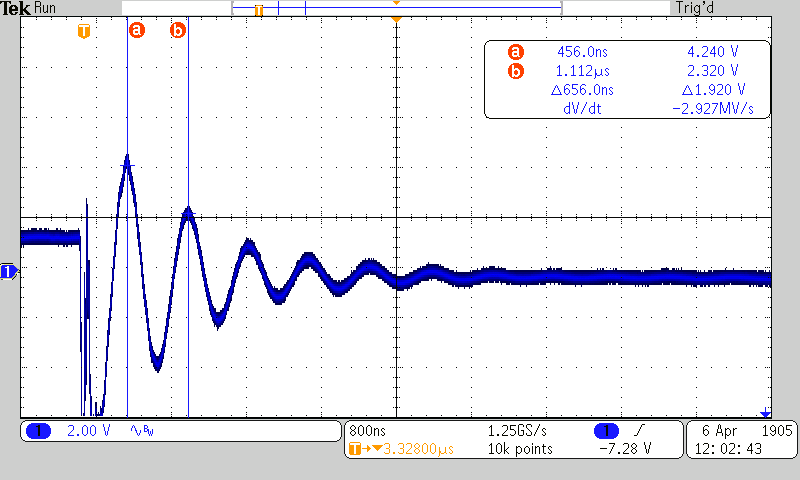
\includegraphics[width=0.6\textwidth]{../Pictures/P1/Test/ringing.png}
		\caption{Console output.}
		\label{fig:ringing}
	\end{center}	
\end{figure}


The simulation result of the inductor and output voltage ripple have the same value as those stated in the system requirement. This means the component have been selected correctly. 
In both cases, the experimental results for the ripples are smaller than in the simulation. The used output capacitor is oversized by a factor of ten and thus the ripple should be ten times smaller than the calculated one, as shown in table \ref{tab:ripple}. Also, the output ripple was tested in buck mode instead of boost mode due to malfunctioning of MOSFET 4 driver. This is not the worst case for the output voltage ripple.

\begin{table}[H]
	\centering
	\begin{tabular}{|>{\centering}p{3.5cm}|p{3cm}|p{3cm}|p{3cm}|}
		\hline
		\rowcolor{lightgray} \textbf{} & \textbf{Requirement} & \textbf{Simulation}  & \textbf{Experiment}   \tabularnewline \hline
		$\Delta V_{in}$ & 0.1\% & 0.099\% & - \tabularnewline \hline
		$\Delta I_{L}$ & 10\% & 10.0\% & 9.86\% \tabularnewline \hline
		$\Delta V_{out}$  & 0.5\% & 0.502\% & 0.055\% \tabularnewline \hline
	\end{tabular}
	\caption{Voltage and current ripple.}
	\label{tab:ripple}
\end{table}

\subsection{Maximum power point tracking} \label{MPPT_discussion}

The proposed Perturb and Observe algorithm was simulated and also tested in the PV lab to show its real performance. The simulation was implemented in PLECS beccause this software allows to program easily the C-code for the MPPT algorithm. The results obtained showed MPPT's efficiencies higher than 99\% for the different levels of irradiance and temperature. As mention in previous chapters, the MPPT algorithm was designed with the objective of increasing the power generated by the PV panel. This was achieved in simulations together with fast MPP tracking and low oscillations around the MPP. 

Table \ref{tab:comparisonMPPT} shows the simulated results together with the experimental results for STC. The experimental results show that the MPPT's efficiency is higher than 97\%. Therefore, the performance of the proposed P\&O algorithm is in the rate of the most common MPPT algorithm which varies between 96\% and 99\% \cite{MPPTResearch}. For the case of the conventional P\&O algorithm, the MPPT's efficiency is around 96\% \cite{MPPTResearch}. Hence, the modifications applied to the conventional P\&O algorithm allowed to improve the MPPT's performance. 

\begin{table}[H]
	\centering
	\begin{tabular}{|>{\centering}p{2.3cm}|>{\centering}p{2.3cm}|>{\centering}p{2.3cm}|>{\centering}p{2.3cm}|>{\centering}p{2.3cm}|}
		\hline
		\rowcolor{lightgray}\multicolumn{5}{|l|}{ \textbf{Standard Test Conditions (STC)}} \\ \hline
		 \rowcolor{lightgray} & \multicolumn{2}{|c|}{ \textbf{Buck Mode}} & \multicolumn{2}{|c|}{ \textbf{Boost Mode}} \tabularnewline \hline
		\rowcolor{lightgray} \textbf{} & \textbf{Simulation}  & \textbf{Experiment} & \textbf{Simulation}  & \textbf{Experiment}  \tabularnewline \hline
		$\eta_{MPPT}$ & 99.96 \% & 97.72 \% & 99.82 \% & 97.32 \% \tabularnewline \hline
		$t_{MPPT}$ & 2 s & 10 s & 4 s & 21 s \tabularnewline \hline
	\end{tabular}
	\caption{Simulated and experimental results for the P\&O MPPT algorithm under STC.}
	\label{tab:comparisonMPPT}
\end{table}

Comparing the experimental results with the simulated ones, from table \ref{tab:comparisonMPPT}, it is seen that the time the MPPT takes to reach the MPP is five times higher than in simulation, this is most likely due to noise and ripple on the measurements. On the other hand, by comparing the efficiency of the MPPT algorithm, it is seen that the error is  2.24\% and 2.5\% for buck and boost mode, respectively. With these results, the P\&O algorithm is considered accurate enough to validate its performance under STC.

The second test was performed to observe the behavior of the MPPT algorithm under sudden changes in irradiance and temperature. Table \ref{tab:comparisonMPPTchanges} shows that, in the case of change in irradiance, by keeping constant the temperature to 25$\decC$, the measured MPPT's efficiency is reduced. The maximum error is achieved when the P\&O is tracking the corresponding MPP for 800$W/m^2$. The error is, in this case, 5.92\%. It is also observed that in simulation the response time is much lower than under STC. However, the time ratio between simulation and test is 13.2 in this case. For the sudden change in temperature, by keeping constant the irradiance to 1000$W/m^2$, the MPPT's performance is considerably improved. The maximum error is 1.5\%. Moreover, a faster MPP tracking is achieved in this case. 

\begin{table}[H]
	\centering
	\begin{tabular}{|>{\centering}p{2.3cm}|>{\centering}p{5cm}|>{\centering}p{5cm}|}
		\hline
		\rowcolor{lightgray}\multicolumn{3}{|l|}{ \textbf{Change in irradiance and constant temperature}} \\ \hline
		\rowcolor{lightgray} & \multicolumn{1}{|c|}{ \textbf{Simulation}} & \multicolumn{1}{|c|}{ \textbf{Experiment}} \tabularnewline \hline
		$\eta_{MPPT}$ & From 99.81\% to 99.70\% & From 95.96\% to 93.78\% \tabularnewline \hline
		$t_{MPPT}$ & 0.5 s  & 6.6 s \tabularnewline \hline
		\rowcolor{lightgray}\multicolumn{3}{|l|}{ \textbf{Change in temperature and constant irradiance}} \\ \hline
		\rowcolor{lightgray} & \multicolumn{1}{|c|}{ \textbf{Simulation}} & \multicolumn{1}{|c|}{ \textbf{Experiment}} \tabularnewline \hline
		$\eta_{MPPT}$ & From 99.81\% to 99.90\% & From 99.20\% to 98.40\%
		\tabularnewline \hline
		$t_{MPPT}$ & 2 s  & 4.1 s \tabularnewline \hline
	\end{tabular}
	\caption{Simulated and experimental results for the P\&O MPPT algorithm under sudden change in irradiance (1000-800$W/m^2$) and temperature (25-15$\decC$) in buck mode ($R_{L}=3\Omega$).}
	\label{tab:comparisonMPPTchanges}
\end{table}

\section{Problems and limitations}

During the project some unexpected problems and limitations were discovered. These are described with possible solutions in this section.


%3-Explain main problems and limitations and how are handled. Be succinct, be frank but no apologetic. Explain implications of limitations.
%\subsection{Layout improvement procedure and issues, title to be improved}
%opto <--x-->driver voltage levels?

%inductor saturation and so

%pcb hot points

\subsection{Discontinuous conduction mode}
\label{DCM_Discussion}

\todo{DCM content is here, consider revising location. AT}

According to chapter 5 of "Fundamentals of Power Electronics" \cite{Erickson} "the discontinuous conduction mode (DCM) arises when the switching ripple in an inductor current is large enough to cause the polarity of the applied switch current to reverse". 

In the case of the bidirectional non-inverting buck-boost, the MOSFETs do not stop reverse current flow like diodes would do, this fact makes the system behave in unexpected ways since current is able to flow through the coil in the opposite direction. An example of this could be found when working in buck mode with a very low power generation at the PV. In this case, since the current is not blocked by a diode, it falls bellow zero, current would then start flowing out of the output capacitor and into the inductor, charging it in the opposite direction. When MOSFET 1 is ON, the current then flows through it and into the input capacitor and the PV. 

The boundaries for entering this DCM scenario are dependent on the PV power and on the voltage at the output. As the power generated by the PV decreases due to a change on the environmental conditions, the current also drops. Under these circumstances there is a limit for the inductor to work in continuous conduction mode (CCM). If this limit is exceeded, the inductor would undergo negative current.

However, the conditions for the inductor to enter DCM are very exceptional. In the figures \ref{DCM_3D_Buck} and \ref{DCM_3D_Boost}, the inductor distance to reach DCM under different output voltages and generated powers is shown. The power plotted has been calculated at a constant temperature of $15\dec C$ and at changing irradiance from $5W/m^2$ to $100W/m^2$. All the calculations have been performed assuming MPP.
The z-axis of the plot represents the distance from zero to the lower peak of the current ripple.

In the figures, it is seen how DCM is only reached under very limited conditions, with very low power generated in the PV. Due to this, when the behavior is present, the current is very low and it is unlikely that the PV would be damaged from this issue \todo{sure¿?}. Nevertheless, it is a topic of great consideration for further research.

\begin{figure}[H]
	\begin{center}
	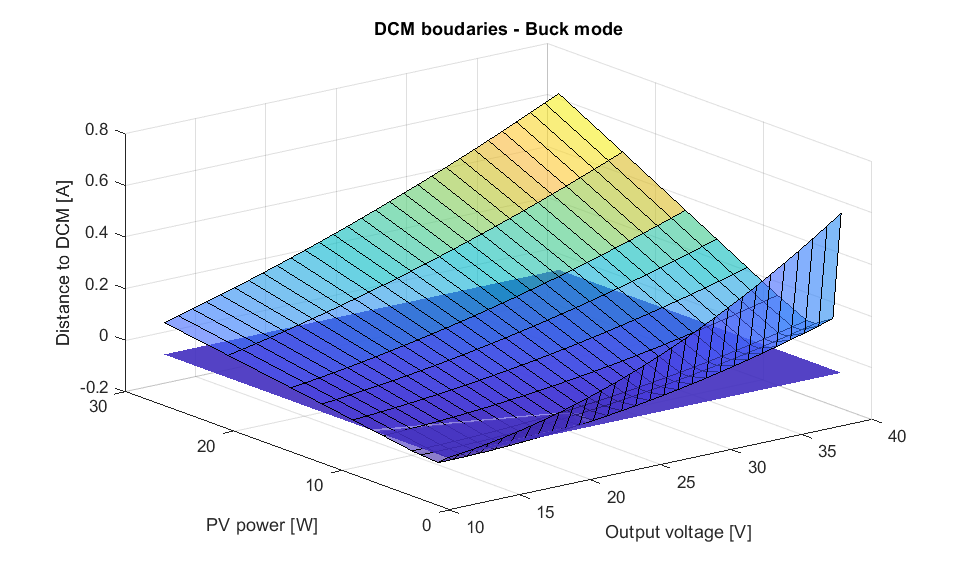
\includegraphics[width=1\textwidth]{../Pictures/Buck_DistanceToDCM.png}
		\caption{Boundary conditions for DCM - Buck mode.}
		\label{DCM_3D_Buck}
	\end{center}	
\end{figure}



\begin{figure}[H]
	\begin{center}
		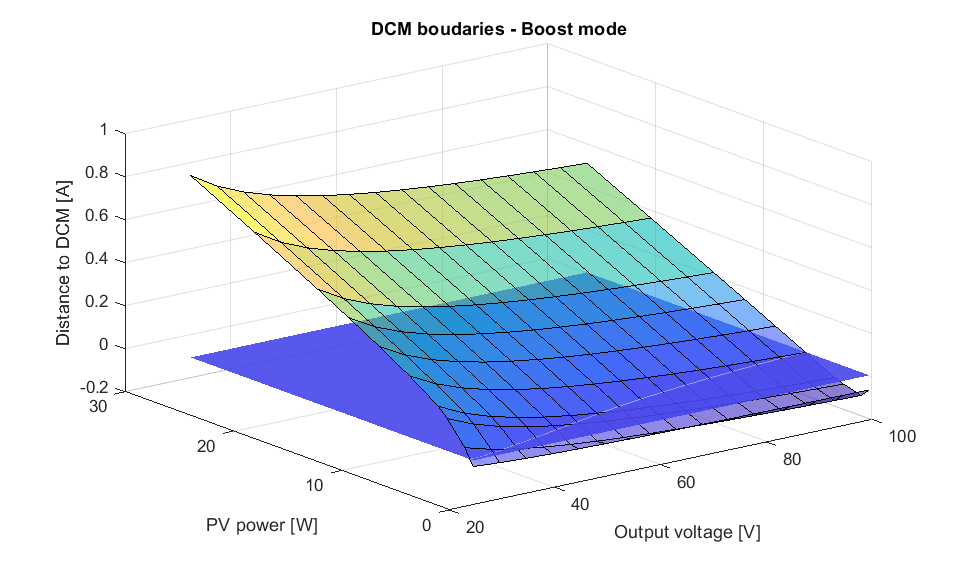
\includegraphics[width=1\textwidth]{../Pictures/Boost_DistanceToDCM.png}
		\caption{Boundary conditions for DCM - Boost mode.}
		\label{DCM_3D_Boost}
	\end{center}	
\end{figure}




\subsection{Output capacitor} \label{output_cap_discussion}	
The output capacitor was sized 10 times to big, because of a calculation error. This meant that the voltage ripple at the output was in the range of 10 times lower than the requirements stated. To achieve an output ripple voltage at $0.5\%$ with a margin at $20\%$, a $100\mu F$ capacitor should be used. A suggestion could be this $100 \mu F$ electrolytic capacitor from Panasonic \cite{new_out_cap_datasheet}.

\subsection{Inductor}
\label{Coil problems}
Since the scope of the project was the validation of the converter, it was decided to implement an existing inductor. A coil was then selected with an approximate inductance of slightly over $1mH$.
The PCB was then designed for this initial inductor. However, after some  tests under high currents it was shown that the coil was not maintaining its inductance due to saturation of the core. Also, it was reaching temperatures over $100\dec C$. The inductance was then tested under different currents and the behavior was verified as shown in figure \ref{Coil comparison}.

It was then decided to implement another inductor which would satisfy the requirements in all cases. The same tests were performed for the new inductor and it was shown that it would fulfill the requirements without problems. 
Also, some thermal tests were performed on the new inductor. With a constant current of $10A$, it shows a maximum temperature of $60\dec C$ after 10 minutes.

\begin{figure}[H]
	\begin{center}
		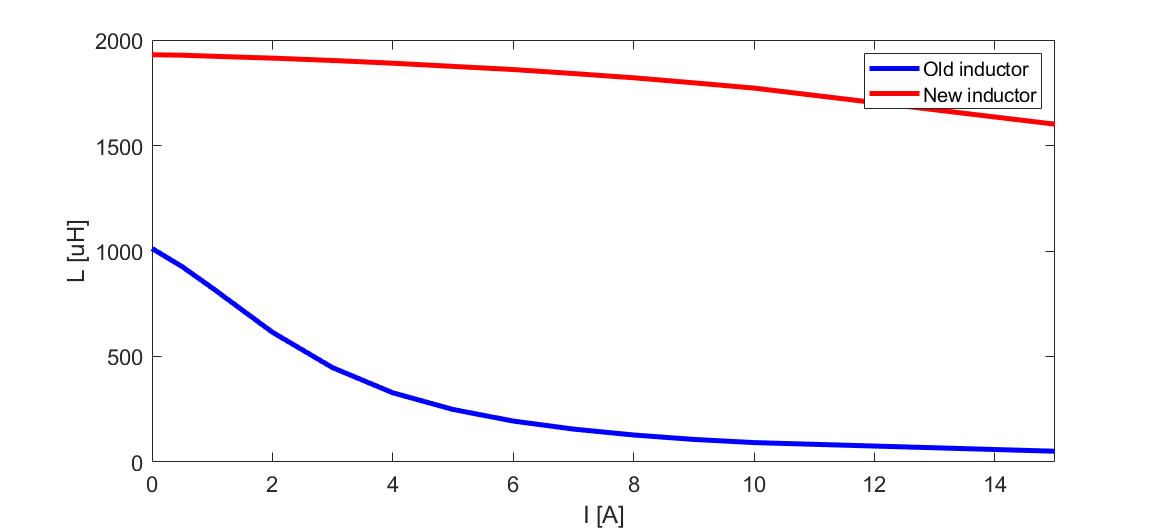
\includegraphics[width=1\textwidth]{docs/discussion/CoilTests/CoilComparison50kHzV2.png}
		\caption{Inductor comparison under changes on current flow (50kHz).}
		\label{Coil comparison}
	\end{center}	
\end{figure}

However, the size and weight of the new inductor are much higher than those of the previous one. This means that the footprint designed is not valid for the new coil and it hangs loose outside the PCB.



\subsubsection{Drivers and optocouplers}  \label{driver}

The control signal is generated by the control platform, which consists on a Plexim RTbox. In order to provide galvanic isolation between the converter and the control signal generator, optocouplers are used. The chosen optocoupler is the ACPL-P302. This optocoupler includes output signal circuitry which allows saving a pull-up or pull-down resistor. The IC is not an open collector device. Its main features might be seen at \ref{opto_features}.

\begin{table}[H]
	\centering
	\begin{tabular}{|p{6cm}|>{\centering}p{8cm}|}
		\hline
		\rowcolor{lightgray}\multicolumn{2}{|l|}{ \textbf{Maximum ratings}} \\ \hline
		Supply voltage & 35 [V]  \tabularnewline \hline
		Average input current & 25 [mA]  \tabularnewline \hline
		Peak output current & 0.4 [A]  \tabularnewline \hline
		\rowcolor{lightgray}\multicolumn{2}{|l|}{ \textbf{Other values of interest}} \\ \hline
		Input forward voltage & 1.5 [V]  \tabularnewline \hline
		Package & SSOIC6  \tabularnewline \hline
	\end{tabular}
	\caption{Optocoupler figures of merit.
	\cite{opto_datasheet}}
	\label{opto_features}
\end{table}

The signal from the optocoupler has to be amplified in order to drive the switches. The driver provides voltage amplification and current capability. The chosen IC to perform the task is NCP81074B. Find in table \ref{driver_features} its main features. 

\begin{table}[htbp]
	\centering
	\begin{tabular}{|p{6cm}|>{\centering}p{8cm}|}
		\hline
		\rowcolor{lightgray}\multicolumn{2}{|l|}{ \textbf{Maximum ratings}} \\ \hline
		Supply voltage & 24 [V]  \tabularnewline \hline
		Output current (pulse < 0.5 $\mu$s) & 10 [A]  \tabularnewline \hline		
		Reverse current (pulse < 1 $\mu$s) & 10 [A]  \tabularnewline \hline
		Input signal voltage & -6 to 24 [V]  \tabularnewline \hline
		\rowcolor{lightgray}\multicolumn{2}{|l|}{ \textbf{Other values of interest}} \\ \hline
		Output resistance & 0.4 [$\Omega$]  \tabularnewline \hline
		Package & SOIC8  \tabularnewline \hline
	\end{tabular}
	\caption{Driver figures of merit.
		\cite{driver_datasheet}}
	\label{driver_features}
\end{table}

The MOSFET is a voltage controlled device, the relationship between $V_{GS}$ and $V_{th}$ sets the drain to source maximum current, as seen in figure \ref{ids_vgs}.

\begin{figure}[htbp]
	\begin{center}
		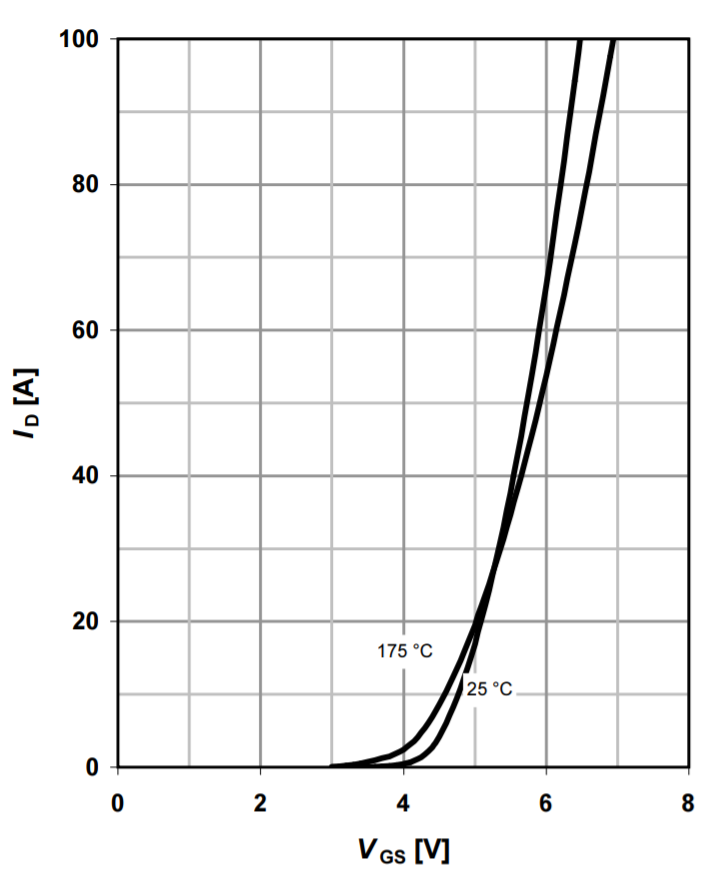
\includegraphics[width=0.4\textwidth]{../Pictures/P1/Component_sizing/ids_against_vgs.png}
		\caption{Drain to source current against gate to source voltage $(V_{DS} > 2 \cdot I_{D}\cdot R_{DSon}) $.}
		\label{ids_vgs}
	\end{center}
\end{figure}

The dynamics of the switching can be modelled as a RC circuit, see figure \ref{mosfet_rc_gate}. Both $R_{driver \; out}$ and $R_{MOSFET}$ are directly obtained from the components' data sheets, $C_{iss}$ is also available in the MOSFET data sheet as input capacitance.



\begin{figure}[H]
	\begin{center}
		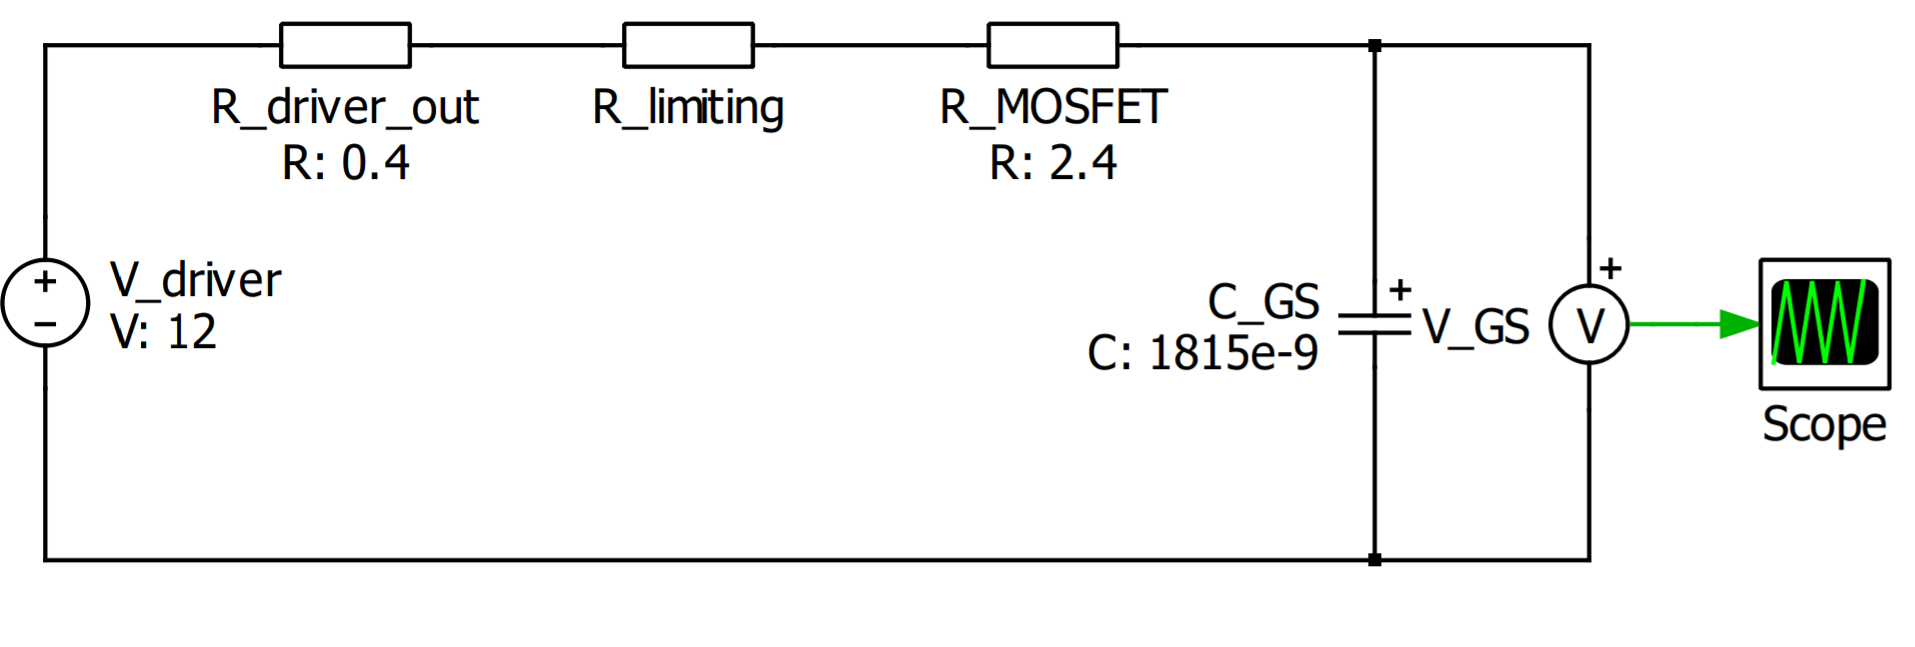
\includegraphics[width=0.8\textwidth]{../Pictures/P1/Component_sizing/driver_resistor_sizing.png}
		\caption{Simplified circuit used to model the MOSFET switching dynamics.}
		\label{mosfet_rc_gate}
	\end{center}	
\end{figure}

The time where the gate capacitor voltage reaches the threshold voltage produces a propagation delay from the driver output to the actual beginning of the MOSFET switching. In order to size the limiting resistor of the RC circuit, a time constraint was needed. This time constraint was arbitrarily set in relation with the switching frequency as described in equation \ref{time_constraint}. The 0.1\% constraint results in a limiting resistor of 20 $\Omega$. The average power dissipation, according to simulation, is 13 mW. This value is well under the power rating of the used SMD resistor with 1206 package, which is 250 mW. However the peak power dissipation was also considered, as it is relatively high. According to simulation, the peak is equal to 5.4 W, see figure \ref{gate_resistor_power_dissipation}. Although this value exceeds the resistor power rating, some manufacturers agree that the peak power dissipation in pulses shorter than 10 $\mu$s using 1206 resistors is 19 W \cite{pulse_withstanding_chip_resistors}, \cite{gate_driver_design_infineon}. Then the peak power dissipated shouldn't harm the component. Once the prototype is built, the thermal behaviour of the component is analysed with a thermal camera. \todo{did we get to do this?}

\begin{equation} \label{time_constraint}
t_{delay} = t\big\rvert_{V_{GS} = V_{th}} =\frac{T_{sw}}{1000} = 0.1 \% \;\; of \;\; T_{sw} = 20 \; ns
\end{equation}


\begin{figure}[H]
	\begin{center}
		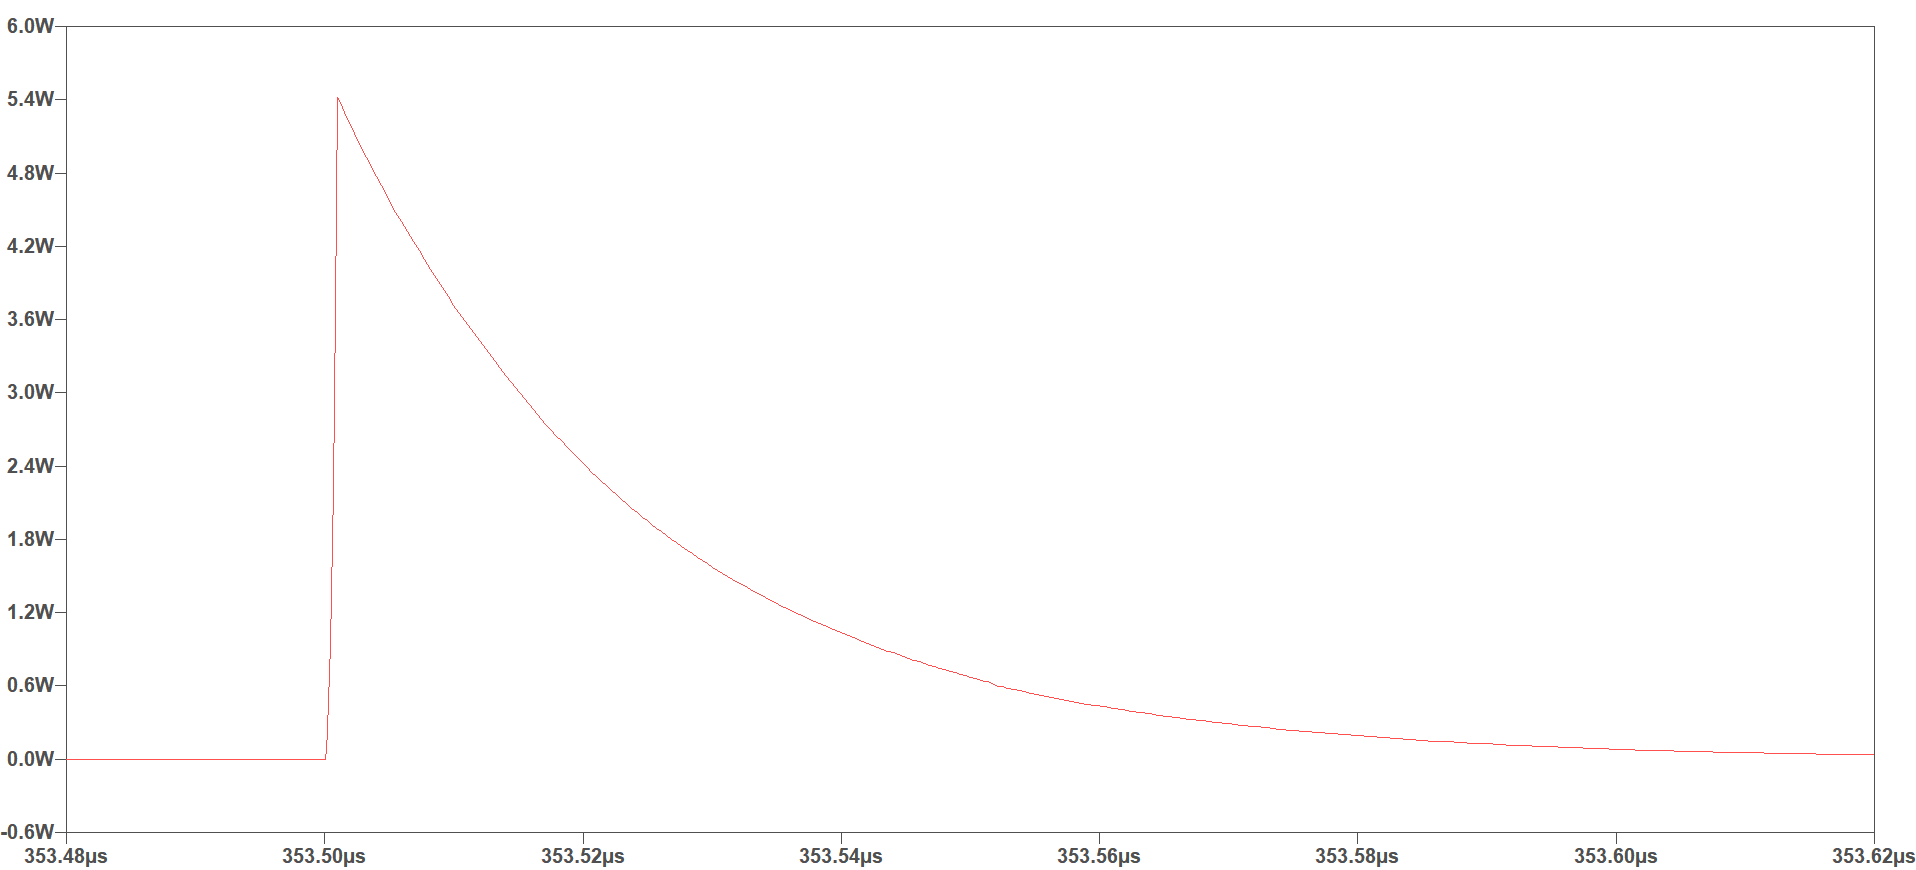
\includegraphics[width=1.15\textwidth]{../Pictures/P1/Component_sizing/Gate_resistor_power_dissipation.png}
		\caption{Detail of the power dissipated at R\_limiting during MOSFET turn-on.}
		\label{gate_resistor_power_dissipation}
	\end{center}	
\end{figure}
 
The implemented topology has the peculiarity that two MOSFETs' sources are not directly connected to ground. As explained previously, it is the Gate to Source voltage that determines whether the transistor is conducting or not. In order to get a floating voltage in the high side drivers, one option is to have isolated supplies for those drivers. The ground of this isolated supplies will be tied to the low side MOSFET's drain. More explanation regarding the isolated supplies might be found at \ref{power_supplies}.

In case that the drivers were damaged, the residual voltage of the transistor's gate might become undefined, then, in order to ensure that the switch is off, a pull down resistor is added between the gate and the source of the transistor. This resistor has been sized to 1 M$\Omega$, which discharges the gate voltage from 12 V to below its threshold in less than 3 ms.


\subsection{MPPT algorithm}
The embedded control system requires the algorithm to work properly. During the development process, the code might not behave as intended. A common way of supporting the debugging process consists of the use of breakpoints. 
The code can then be stopped and the variables' value might be read. However, this feature is not supported by the used platform. In the case of controlling physical systems, the use of breakpoints would be limited to simulation. Then alternative techniques had to be used. 
The adopted approach consisted on outputting the FSMs' state and relevant values for the current state at every code execution loop. 
The 'Timestamp' field is specially important during simulation in order to track events at specific times. See figure \ref{console_output}.

\begin{figure}[htbp]
	\begin{center}
		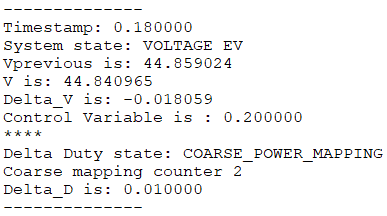
\includegraphics[width=0.5\textwidth]{../Pictures/P1/Discussion/console_output.png}
		\caption{Console output.}
		\label{console_output}
	\end{center}	
\end{figure}

In initial implementations of the control algorithm, the voltage evaluation was performed in the state after the duty cycle change. 
After this change, the system experiences a transient stage where the input voltage and inductor current evolve into the new steady state value. If these variables are read during the transient, the control might infer that the PV panel is in a location of the P-V curve different from where it actually is. 
The MPPT becomes noisier under this scenario. In order to address this issue, an additional waiting state was added to the FSM governing the system. 
Another solution to the issue would be to decrease the MPPT algorithm periodicity. However this solution would lead to a decrease in system's responsiveness. This drawback might be bearable by implementing a voltage controller aside from the MPPT.  

The noise in measured signals highly influenced the algorithm performance. This noise was addressed by software low pass filtering. The filter caused a dramatic improvement in signal acquisition and system response, further details are explained in the next section.

In order to develop a completely reliable algorithm further testing must be performed. These tests require more advanced debugging information than the console output previously shown. RT Box allows SPI communication but the testing activities would still be limited to black-box techniques. In order to reach white-box testing, the implementation would require a microcontroller instead of the RT Box. If that was the case, the variables' value might be directly accessed with a debugger. Also in the case of black-box testing, the signals are sent with a known and fixed latency by the microcontroller, which is not the case when using PLECS's console.

The implemented algorithm has more advanced functions than the simplest implementation found in introductory application notes from manufacturers \cite{AN1521_MC}. 
Among the advanced functions, threshold parameters are tunable, waiting for the PV to reach open circuit voltage or variable perturb step, among others. However, these additional features add difficulty to the tests and code comprehension. Under the development of a commercial product, it might be desirable to limit the features in order to decrease test and validation cost. The decrease of the perturb variable consists of a FSM with 5 states with a weak coupling with the main FSM.

The proposed implementation has some variables which might be further optimized, like the initial value or the threshold to decrease the perturb step. 


\subsection{Software filter}
Although the voltage and current measurement is hardware filtered, the signal read by the control system was noisy. This affected the MPPT algorithm, disturbing its ability to reach the MPP. There are many techniques in order to address noise issues, the used technique consists in the use of a low pass digital filter. The result can be seen in \ref{software_filter}. It consists of a single pole low pass filter. Its corner frequency is set as the same of the hardware filters, 50 Hz. In order to design the software filter, explanations from \cite{digital_filter} have been followed.

First, the execution frequency of the filter $f_{filter}$ is defined. It is set to $20 kHz$, this frequency is low enough to have a low CPU consumption, according to RT Box estimation. Now, $\tau$ must be calculated, as seen in equation \ref{tau_calculation}. 

\begin{equation} \label{tau_calculation}
\tau= \dfrac{1}{2\pi \cdot f_c} = 3.18 ms
\end{equation}

The implemented single pole low pass filter has the recursive equation explained in \ref{filter_recursive_eq}. The parameters $a_0 $ and $b_1$ must be found. 

\begin{equation} \label{filter_recursive_eq}
y_n= x_n \cdot a_0 + y_{n-1} \cdot b_1
\end{equation}

First, $b_1$ is calculated as explained in \ref{b1_calc}. Then $a_0$ is easily calculated as shown in \ref{a0_calc}.

\begin{equation} \label{b1_calc}
b_1=  e^{\frac{-1}{f_{filter} \cdot \tau}} = e^{\frac{-1}{20 \times 10^{3} \cdot 3.18 \times 10^{-3}}} = 0.9843
\end{equation}

\begin{equation} \label{a0_calc}
a_0=  1 - b_1 = 0.0156
\end{equation}

The design is validated by analysing the step response of the filter. The result can be seen in figure \ref{step_response_filter}. $\tau$ is confirmed, reaching around $63\%$ of the value in the required time. Cursor one is fixed at the beginning of the step and cursor 2 is set at $0.6327$, the time difference is $3.25 ms$. 

\begin{figure}[H]
	\begin{center}
		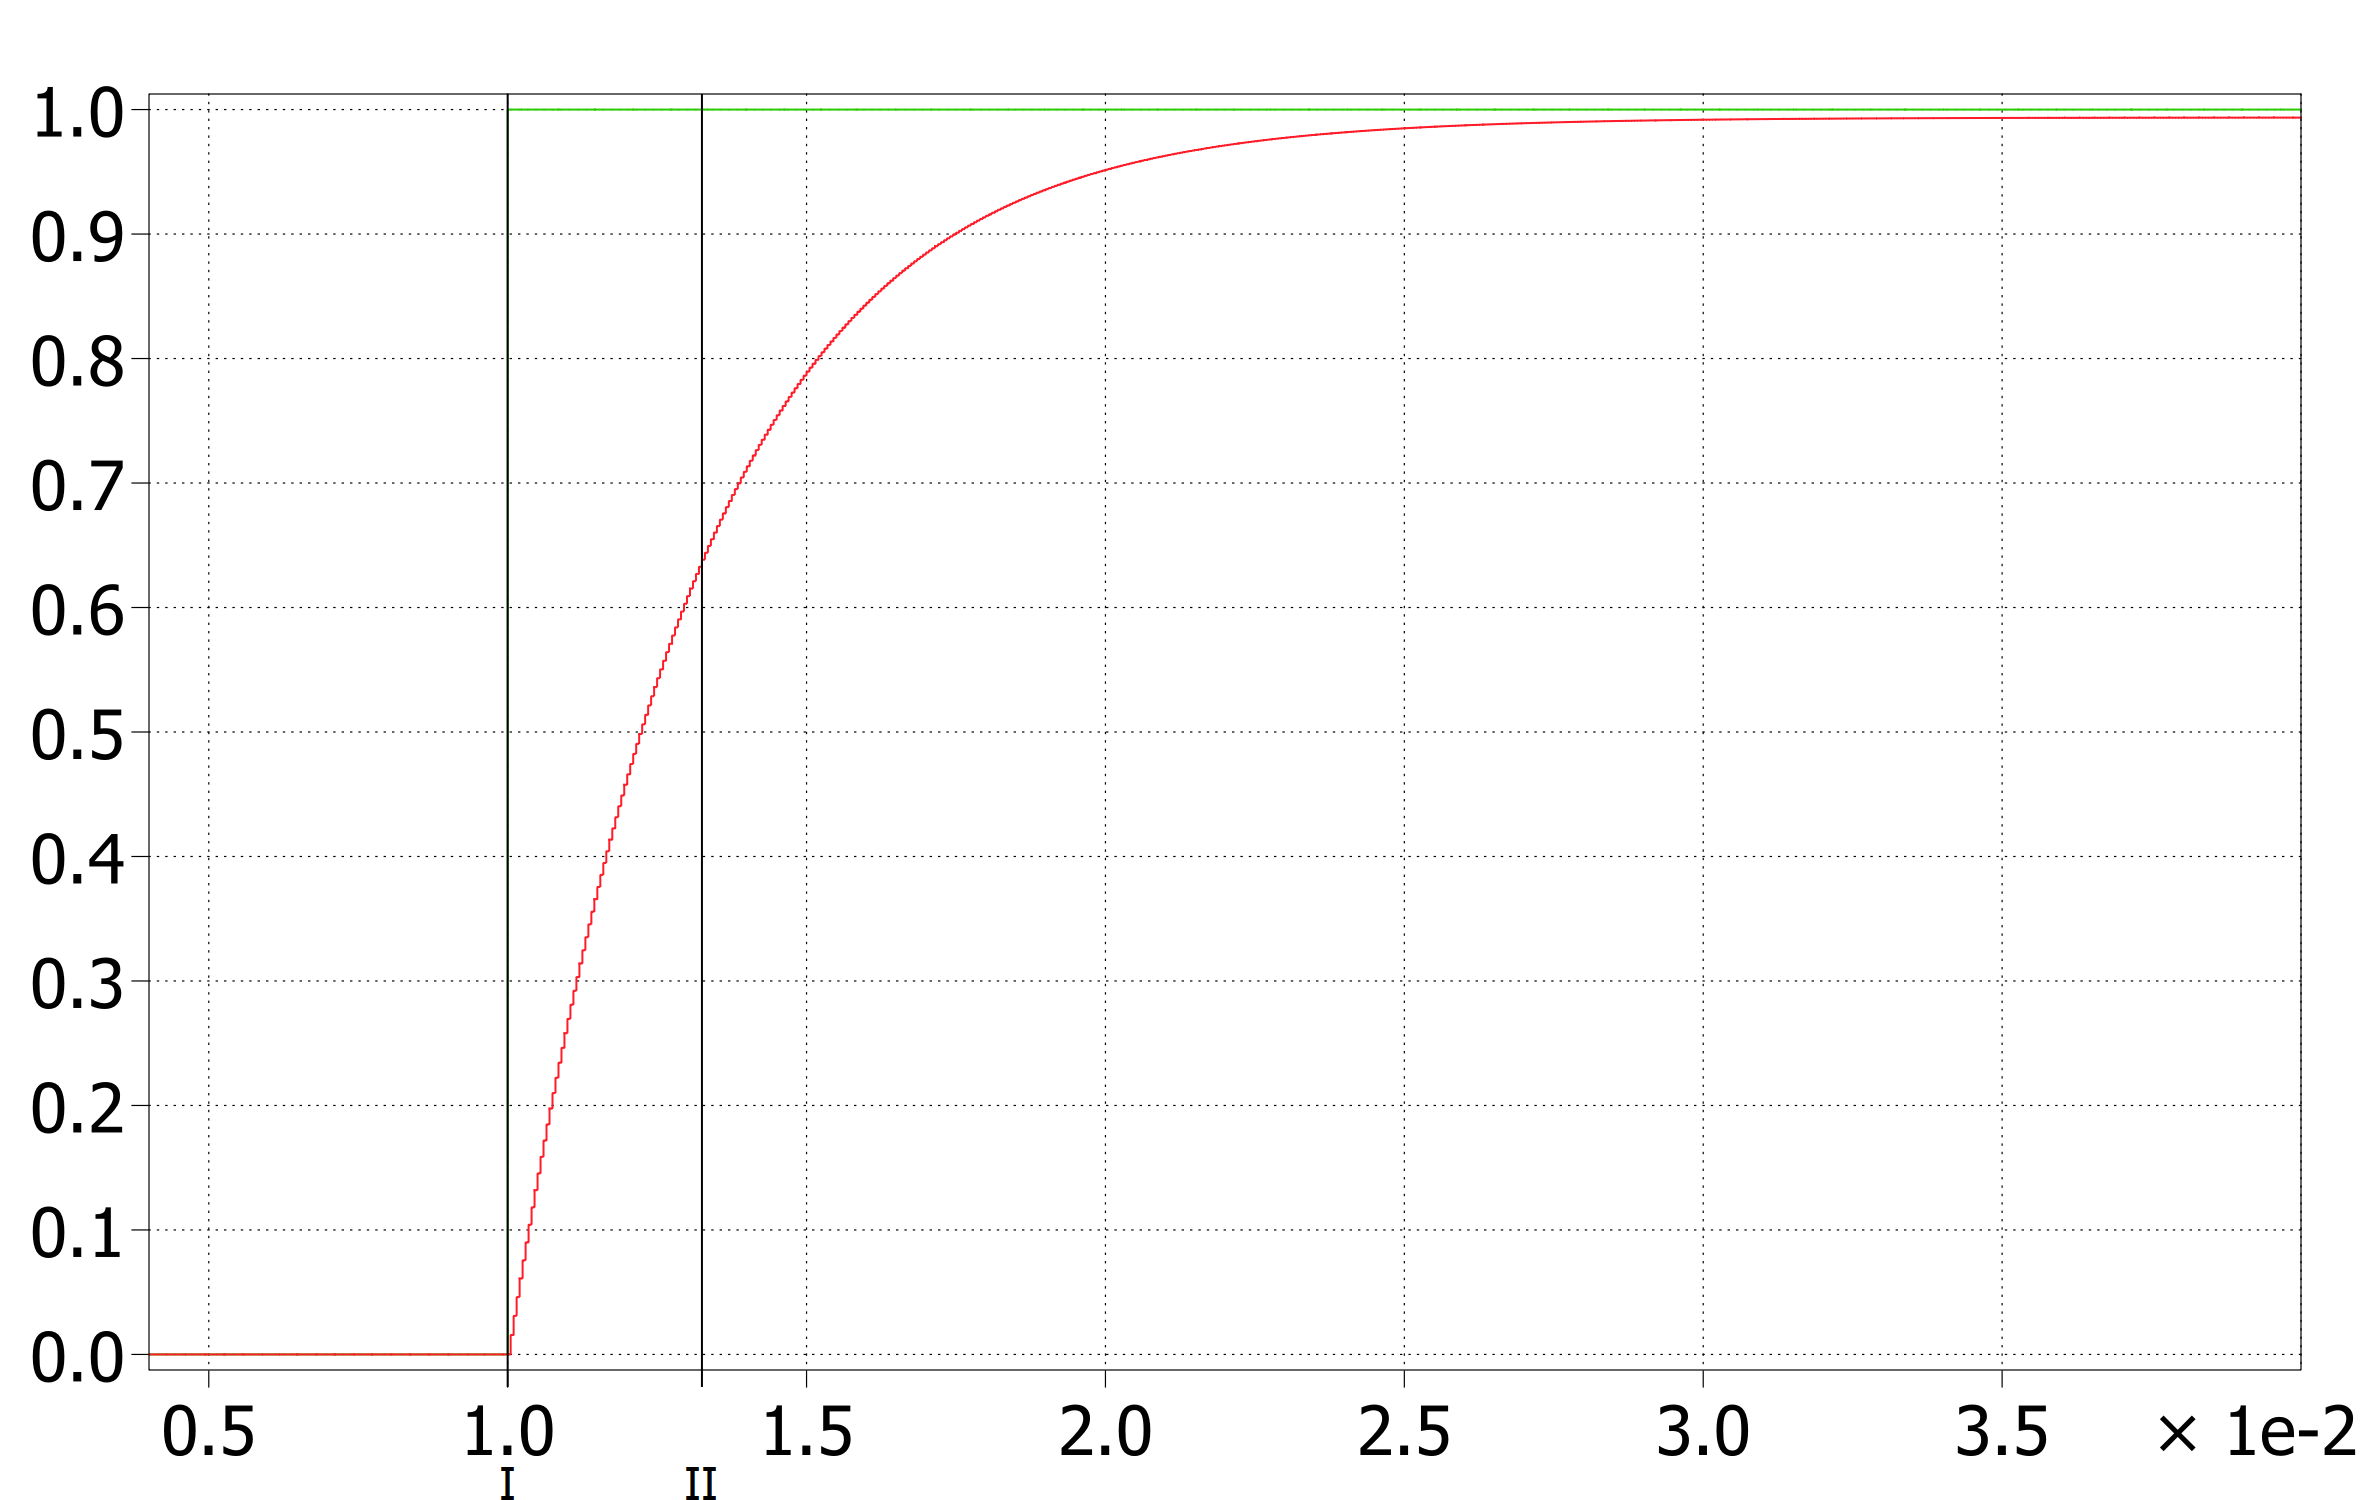
\includegraphics[width=0.7\textwidth]{../Pictures/P1/Discussion/filter_step_response.png}
		\caption{Step response of the designed filter.}
		\label{step_response_filter}
	\end{center}	
\end{figure}


The tested result can be seen in figure \ref{software_filter}.

\begin{figure}[H]
	\begin{center}
		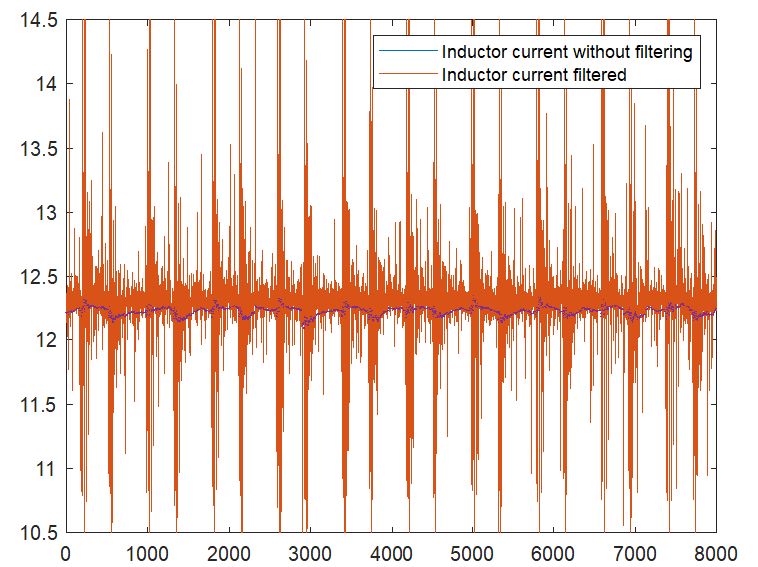
\includegraphics[width=0.8\textwidth]{../Pictures/P1/Discussion/sw_filter_current_new.png}
		\caption{Current measurement against time. Both software filtered (blue) and raw (red) signals can be seen. The filtered signal data points' size has been increased to improve readability.}
		\label{software_filter}
	\end{center}	
\end{figure}

\section{Future work}
This section will describe the planned future work of the project. This includes parts that were prioritized low or Simplified to achieve a working converter. Furthermore it includes improvements that was discovered during both the development and testing period of the project.

%4- Recommendations for future work. Make general statements. Items: a)what study is needed, b)Methods to be used, c)what is needed for that study.

\subsection{MPPT technique}
Even though the P\&O algorithm was implemented, initial research showed that the incremental conductance method could have been a better option.  Further research and simulations will have to be made for comparing the two methods. \todo{Write about what could be gained from changing MPPT, NHF.}

\subsection{V/I controller}


\subsection{Hardware improvements}
In the first iterations of the converter design, the driver circuits have been designed using isolated power supplies for the high side drivers. These are costly both in size and money wise. Because of that it's preferable to implement a bootstrap circuit for the drivers. An option for a driver including bootstrap could be UCC27211 \cite{boot_driver_datasheet}. This includes both a high and low side driver, such that only to IC's are necessary for the converter. The input threshold is below $2.8V$ for both sides, which means that a $5V$ optocoupler could be used for isolation. For cost and size optimization the optocouplers should be one quad optocoupler, instead of four singles. 
 
%bootstrap, change driver to the A version due to voltage levels and then change the optocouupler to a quad version, control system powered from pv-panel, \dots

\subsection{Coil design}
The coil used for the converter is reused from an earlier project. Measurements shows that it's oversized regarding current ratings. To achieve an optimal coil it should be designed for this specific converter. Both the core size and wire diameter depends on the wanted current rating of the converter \cite{underthehood}. Because of this it will be possible to lower both the cost and size of the coil. 

\subsection{Switching frequency limitations}

%\subsection{Component price, system size, optimization needed}
%Component prize and system size will be introduced during the other sections...

\subsection{Efficiency}
The main purpose of the MIC is to maximize the output efficiency of a PV-panel. To achieve that, the efficiency of the converter itself should be maximized. During the tests, the efficiency was measured to \textit{ADD SOME NICE DATA}\todo{Insert measured efficiency, NHF.}. Other papers shows that an efficiency of up to $95-96\%$ should be achievable\cite{underthehood}, \cite{efficient_buckboost}. 




